% basically this is a template file, you should be able to take it and
% start running.

% the philosophy behind this template is that each chapter or
% chapterlike section goes in a separate file and you use the \include
% command to input it into the final document.  The \includeonly
% command can be used so you only need to work on one or two chapters at a
% time (instead of having to either latex the entire book each time or
% losing cross-references and page numbering)

% copy this file and call it something like mythesis.tex

\documentclass[12pt]{report}
% note that the documentclass can take other option such as
% twoside - for double sided printing
% openright - if double side  chapters always start on odd pages
% openany - if double side chapters start on the next page even or odd
% 12pt can be replaced by 11pt

\usepackage{suthesis-2e}

%% load other packages you need

%% uncomment the following and create mythesis-macros.sty for all your
%% own macros.  This keeps this top level file looking fairly neat.
% \usepackage{mythesis-macros}

%% certain types of theses require special title page format.  See the
%% style file for the full list.  An example would be that for some of
%% the language departments. 
% \dualthesis \dept{Asian Languages} \languagemajor{Korean} 
%% or education
% \educationthesis

    \title{}
    \author{}
%\dept{} % default is Computer Science, uncomment for other departments
    \principaladviser{}
% \coprincipaladvisor{}
    \firstreader{}
    \secondreader{}
% \thirdreader{}

%the following command would (if uncommented) allow  only chapter1 and
%chapter2 to be processed
%\includeonly{chapter1,chapter2}

% if you feel real savvy use
% \typein{Now put in includeonly}
% the \typein command stops latex at this point and allows you to type
% in a command such as
% \includeonly{chapter3,chapter5}
% this can save some time and means you don't have to edit this file
% as much.


\begin{document}

 

% first the preface sections.  

% this includes the file preface.tex which should include the
% following commands
% \beforepreface
% \prefacesection{preface}
% body of the preface
\include{preface}

% any other preface sections

% the last preface section (e.g., acknowledgement.tex)
% should look like
% \prefacesection{Acknowledgement}
% body 
% \afterpreface
% Thesis Acknowledgements ------------------------------------------------


%\begin{acknowledgementslong} %uncommenting this line, gives a different acknowledgements heading
\begin{acknowledgements}      %this creates the heading for the acknowlegments


And I would like to acknowledge ...


\end{acknowledgements}
%\end{acknowledgmentslong}

% ------------------------------------------------------------------------

%%% Local Variables: 
%%% mode: latex
%%% TeX-master: "../thesis"
%%% End: 



% now for the body of the thesis, modify the number of these lines as needed

% this includes chapter1.tex which should start with a \chapter{...}
% command 
% \pagebreak[4]
% \hspace*{1cm}
% \pagebreak[4]
% \hspace*{1cm}
% \pagebreak[4]

\chapter{My First Chapter But Note The Numbering ...}
\ifpdf
    \graphicspath{{Chapter1/Chapter1Figs/PNG/}{Chapter1/Chapter1Figs/PDF/}{Chapter1/Chapter1Figs/}}
\else
    \graphicspath{{Chapter1/Chapter1Figs/EPS/}{Chapter1/Chapter1Figs/}}
\fi

\section{First Paragraph}
And now I begin my first chapter here ...

Here is an equation\footnote{the notation is explained in the nomenclature section :-)}:
\begin{eqnarray}
CIF: \hspace*{5mm}F_0^j(a) &=& \frac{1}{2\pi \iota} \oint_{\gamma} \frac{F_0^j(z)}{z - a} dz
\end{eqnarray}
\nomenclature[zcif]{$CIF$}{Cauchy's Integral Formula}                                % first letter Z is for Acronyms 
\nomenclature[aF]{$F$}{complex function}                                                   % first letter A is for Roman symbols
\nomenclature[gp]{$\pi$}{ $\simeq 3.14\ldots$}                                             % first letter G is for Greek Symbols
\nomenclature[gi]{$\iota$}{unit imaginary number $\sqrt{-1}$}                      % first letter G is for Greek Symbols
\nomenclature[gg]{$\gamma$}{a simply closed curve on a complex plane}  % first letter G is for Greek Symbols
\nomenclature[xi]{$\oint_\gamma$}{integration around a curve $\gamma$} % first letter X is for Other Symbols
\nomenclature[rj]{$j$}{superscript index}                                                       % first letter R is for superscripts
\nomenclature[s0]{$0$}{subscript index}                                                        % first letter S is for subscripts

\section{Second Paragraph}
and here I write more ...\cite{texbook}

\subsection{sub first paragraph}
... and some more ...

Now I would like to cite the following: \cite{latex} and \cite{texbook}
and \cite{Rud73}.

I would also like to include a picture ...

\begin{figure}[!htbp]
  \begin{center}
    \leavevmode
    \ifpdf
      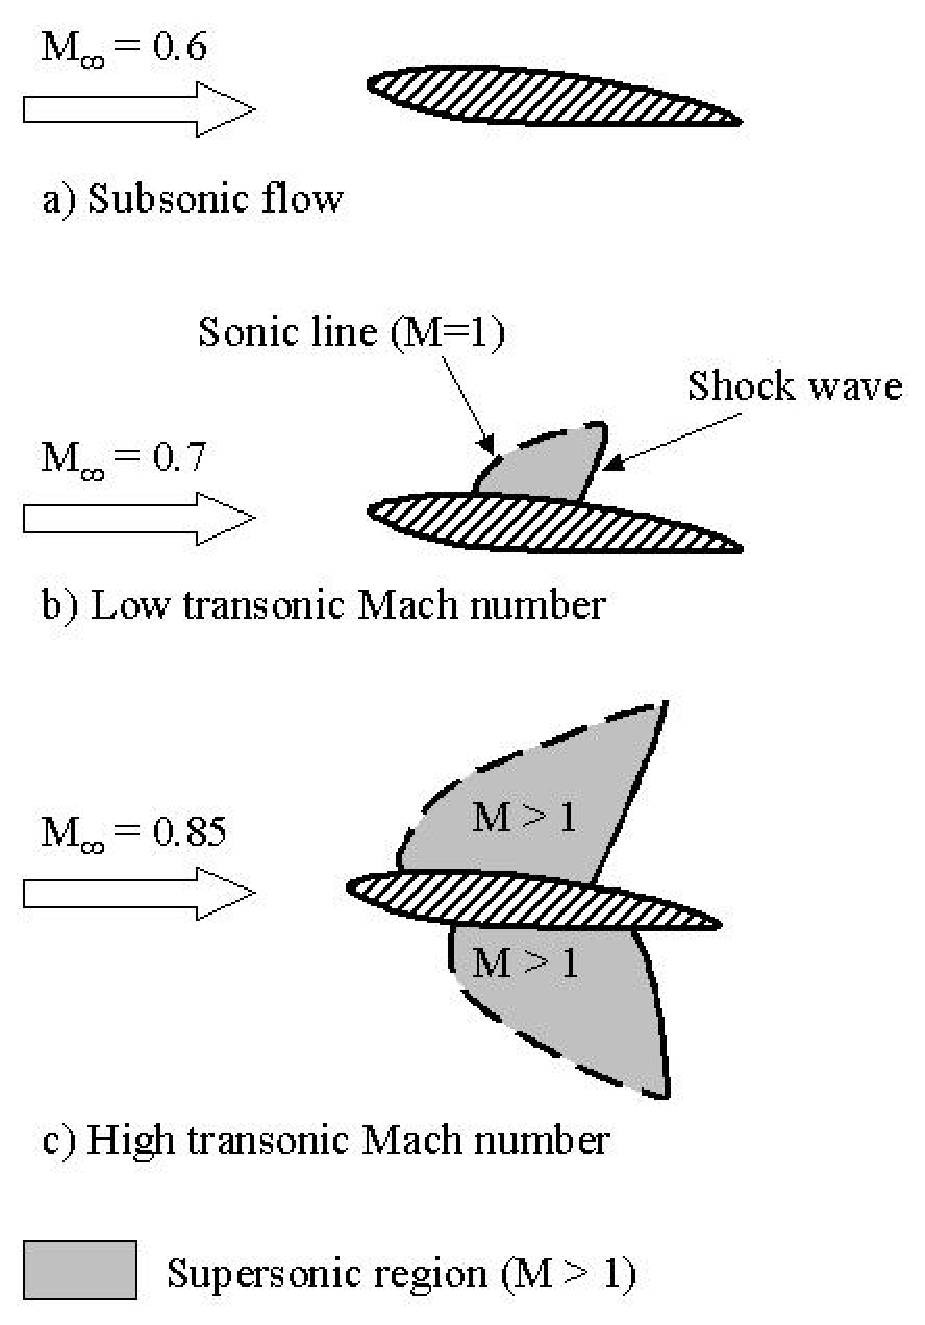
\includegraphics[height=6in]{aflow}
    \else
      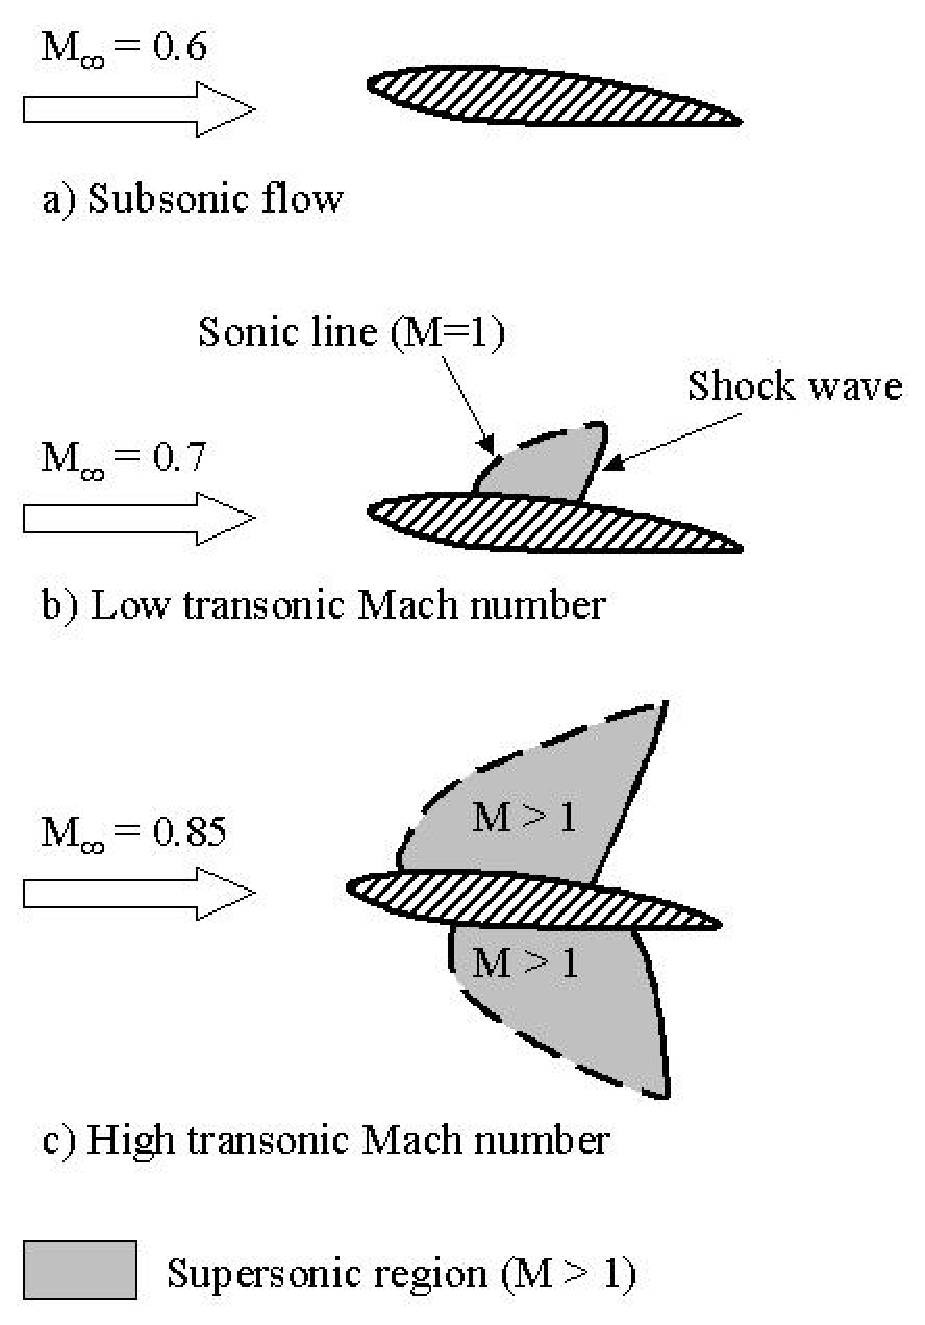
\includegraphics[bb = 92 86 545 742, height=6in]{aflow}
    \fi
    \caption{Airfoil Picture}
    \label{FigAir}
  \end{center}
\end{figure}

% above code has been macro-fied in Classes/MacroFile.tex file
%\InsertFig{\IncludeGraphicsH{aflow}{6in}{92 86 545 742}}{Airfoil Picture}{FigAir}

So as we have now labelled it we can reference it, like so (\ref{FigAir}) and it
is on Page \pageref{FigAir}. And as we can see, it is a very nice picture and we
can talk about it all we want and when we are tired we can move on to the next
chapter ...

I would also like to add an extra bookmark in acroread like so ...
\ifpdf
  \pdfbookmark[2]{bookmark text is here}{And this is what I want bookmarked}
\fi
% ------------------------------------------------------------------------


%%% Local Variables: 
%%% mode: latex
%%% TeX-master: "../thesis"
%%% End: 

\chapter{My Second Chapter}
\ifpdf
    \graphicspath{{Chapter2/Chapter2Figs/PNG/}{Chapter2/Chapter2Figs/PDF/}{Chapter2/Chapter2Figs/}}
\else
    \graphicspath{{Chapter2/Chapter2Figs/EPS/}{Chapter2/Chapter2Figs/}}
\fi

\section{First Section}
\markboth{\MakeUppercase{\thechapter. My Second Chapter }}
And now I begin my second chapter here ...

\section{Second Section}
\markboth{\MakeUppercase{\thechapter. My Second Chapter }}
and here I write more ...

\subsection{first subsection in the Second Section}
... and some more ...

\subsection{second subsection in the Second Section}
... and some more ...

\subsection{third subsection in the Second Section}
... and some more ...

% ------------------------------------------------------------------------

%%% Local Variables: 
%%% mode: latex
%%% TeX-master: "../thesis"
%%% End: 

\chapter{My Third Chapter}
\ifpdf
    \graphicspath{{Chapter3/Chapter3Figs/PNG/}{Chapter3/Chapter3Figs/PDF/}{Chapter3/Chapter3Figs/}}
\else
    \graphicspath{{Chapter3/Chapter3Figs/EPS/}{Chapter3/Chapter3Figs/}}
\fi

\section{First Section of the Third Chapter}
\markboth{\MakeUppercase{\thechapter. My Third Chapter }}{\thechapter. My Third Chapter}
And now I begin my third chapter here ...

\subsection{first subsection in the First Section}
... and some more 

\subsection{second subsection in the First Section}
... and some more ...

\subsubsection{first subsub section in the second subsection}
... and some more in the first subsub section otherwise it all looks the same
doesn't it? well we can add some text to it ...

\subsection{third subsection in the First Section}
... and some more ...

\subsubsection{first subsub section in the third subsection}
... and some more in the first subsub section otherwise it all looks the same
doesn't it? well we can add some text to it and some more and some more and
some more and some more and some more and some more and some more ...

\subsubsection{second subsub section in the third subsection}
... and some more in the first subsub section otherwise it all looks the same
doesn't it? well we can add some text to it ...

\section{Second Section of the Third Chapter}
\markboth{\MakeUppercase{\thechapter. My Third Chapter }}{\thechapter. My Third Chapter}
and here I write more ...

% ------------------------------------------------------------------------


%%% Local Variables: 
%%% mode: latex
%%% TeX-master: "../thesis"
%%% End: 

\include{chapter4}
\include{chapter5}

% and the end material

\appendix

\chapter{Appdx A}

and here I put a bit of postamble ...

% ------------------------------------------------------------------------

%%% Local Variables: 
%%% mode: latex
%%% TeX-master: "../thesis"
%%% End: 

\chapter{Appdx B}

and here I put some more postamble ...

% ------------------------------------------------------------------------

%%% Local Variables: 
%%% mode: latex
%%% TeX-master: "../thesis"
%%% End: 

\include{appendix3}


% bibliography.tex should include either 
% \bibliographystyle{...}
% \bibliography{mythesis}
% or some other way of doing the bibliography
\include{bibliography}

\end{document}

